\documentclass{article}
\usepackage[utf8]{inputenc}
\usepackage[T1]{fontenc}
\usepackage[english]{babel}
\setlength{\parindent}{0pt}
\usepackage{hyperref}
\hypersetup{
    colorlinks=true,
    linkcolor=blue,
    filecolor=magenta,      
    urlcolor=cyan}
\usepackage{graphicx}
\graphicspath{ {./pic/} }
\usepackage{multicol}
\usepackage{lscape}

\usepackage{fourier,amssymb,microtype,amsmath,gensymb}
\newcommand{\R}{\mathbb{R}}
\usepackage{mdframed,caption,xcolor}
\usepackage{tikz,tkz-euclide}

\title{Seminar 4. Elasticity of Substitution}
\author{Xiaoguang Ling \\  \href{xiaoguang.ling@econ.uio.no}{xiaoguang.ling@econ.uio.no}}
\date{\today}

\begin{document}

\maketitle

%%%%%%%%%%%%%%%%%%%%%%%%%%%%%%%%%%%%%%%%%%%%%%%%%%%%%%%%%%%%%%%%%%%%%%%%%%%%%%%%%%%%%%%%%%%%%%
\begin{mdframed}[backgroundcolor=blue!20,linecolor=white]

This review part is to help you to understand Elasticity of Substitution step by step.
It contains the following key points:

\begin{enumerate}
\item The |slop| of indifference curve is \textbf{Marginal Rate of Substitution} ($MRS$);
\item $MRS$ shows the relative importance of the two commodities;
\item The relationship between $MRS_{12}$ and $\frac{x_2}{x_1}$ shows the \textbf{substitution relationship} between the two commodities;
\item The relationship between $MRS_{12}$ and $\frac{x_2}{x_1}$ can be expressed by \textbf{Elasticity of Substitution} $\sigma_{12}$
\end{enumerate}

After this part you will understand:

\begin{enumerate}
\item $\sigma_{12} = 0 \iff$ Leotief preference
\item $\sigma_{12} = constant \iff$ CES
\item $\sigma_{12} = + \infty \iff$ Perfect substitution
\end{enumerate}

Note that I will use MRS instead of MRTS by default in this part, because we have spent more time on consumer theory and MRS
can be easily generalized to MRTS.
%%%%%%%%%%%%%%%%%%%%%%%%%%%%%%%%%%%%%%%%%%%%%%%%%%%%%%%%%%%%%%%%%%%%%%%%%%%%%%%%%%%%%%%%%%%%%%

\section{Substitution along an indifference curve}
\begin{center}
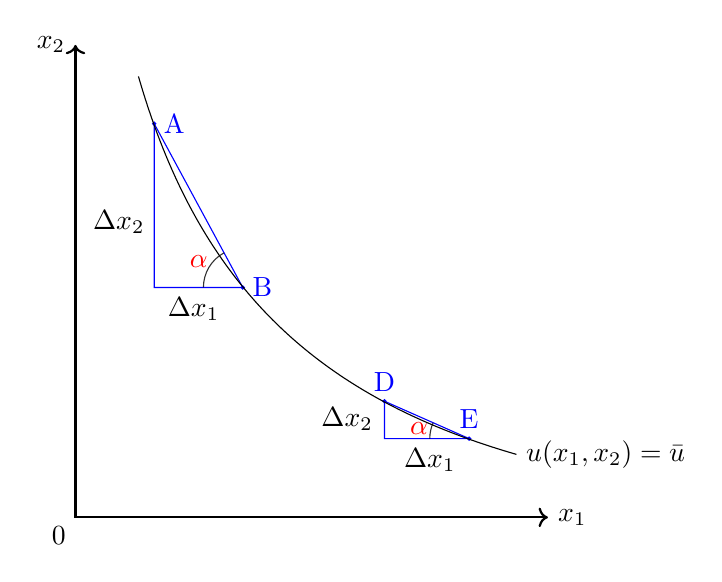
\begin{tikzpicture}[scale=0.5]

\draw[thick,<->] (0,12) node[left]{$x_2$}--(0,0)--(12,0) node[right]{$x_1$};
\node [below left] at (0,0) {$0$};

% \draw(2,9.44)--(4,5.84);
% \draw(9.44,2)--(5.84,4);

% \node[right] at (3.05,7.7) {$x^1$};
% \draw[fill] (3.05,7.56) circle [radius =0.04];
% \node[right] at (7.5,3.3) {$x^2$};
% \draw[fill] (7.56,3.05) circle [radius =0.04];

% \tkzDefPoint(2,9.44){A}
% \tkzDefPoint(4,5.84){B}
\tkzDefPoint(2,10){A}
\tkzDefPoint(4.25,5.84){B}
\tkzDefPoint(2,5.84){C}
\node[right,blue] at (A) {A} ;
\draw[fill,blue] (A) circle [radius =0.04];
\node[right,blue] at (B) {B} ;
\draw[fill,blue] (B) circle [radius =0.04];

\draw [blue] (A)--(B)--(C)--cycle;
\tkzMarkAngle[fill=yellow, opacity=0.8](A,B,C)
\tkzLabelAngle[pos= 1.3,red](A,B,C){$\alpha$}

% \draw [thick,blue] (A) -- (2,10);
% \draw [thick,blue] (B) -- (4.25,5.84);

\node[left] at (2,7.5) {$\Delta x_2$};
\node[below] at (3,5.84) {$\Delta x_1$};

% \tkzDefPoint(5.84,4){D}
% \tkzDefPoint(9.44,2){E}
\tkzDefPoint(7.85,2.95){D}
\tkzDefPoint(10,2){E}
\tkzDefPoint(7.85,2){F}
\draw [blue] (D)--(E)--(F)--cycle;
% \draw [thick,blue] (D) -- (5.84,4.25);
% \draw [thick,blue] (E) -- (10,2);
\node[above,blue] at (D) {D} ;
\draw[fill,blue] (D) circle [radius =0.04];
\node[above,blue] at (E) {E} ;
\draw[fill,blue] (E) circle [radius =0.04];

\tkzMarkAngle[fill=yellow,opacity=0.8](D,E,F)
\tkzLabelAngle[pos= 1.3,red](D,E,F){$\alpha$}

\node[left] at (7.8,2.5) {$\Delta x_2$};
\node[below] at (9,2) {$\Delta x_1$};

\draw(1.6,11.2) ..controls (3.1,6) and (6,3.1) .. (11.2,1.6) node[right]{$u(x_1,x_2)=\bar{u}$};

\end{tikzpicture}
\captionof{figure}{You have to give up $\Delta x_2$ to consume 1 more $\Delta x_1$}
\label{fig:margin}
\end{center}
\vspace{2mm}


When we move along $u(x_1,x_2)=\bar{u}$, we can observe the following facts:
\begin{itemize}
\item The small increase of $x_1$ (i.e. $\Delta x_1$) is always followed by some small decrease of $x_2$ (i.e. $\Delta x_2$). Angle $\alpha$ reflects how much you have to give up (substitute).

\item $\alpha = - \frac{\Delta x_2}{\Delta x_1}$ depends on the relative amount of $x_1$ and $x_2$, i.e. $\frac{x_2}{x_1}$ (Note $\Delta x_2$ is negative here).
\end{itemize}

\textbf{Intuition}: To keep utility the same, you need to give up $\Delta x_2$ to consume $\Delta x_1$. 

\vspace{4mm}

\textbf{Two questions:}

\begin{itemize}
\item How to calculate $\alpha = - \frac{\Delta x_2}{\Delta x_1}$ ?
\item How to describe the relationship between $\alpha$ and $\frac{x_2}{x_1}$ ?
\end{itemize}
%%%%%%%%%%%%%%%%%%%%%%%%%%%%%%%%%%%%%%%%%%%%%%%%%%%%%%%%%%%%%%%%%%%%%%%%%%%%%%%%%%%%%%%%%%%%%%

\section{Marginal Rate of Substitution (MRS)}

When $x_1$ increases one very small unit, we define $\angle \alpha$ as Marginal Rate of Substitution (MRS). 

$$MRS = \alpha = - \frac{\Delta x_2}{\Delta x_1}$$

We can calculate $\alpha$  in the following 2 ways:

\vspace{4mm}

\textbf{Method 1 (2-D thinking)}

When line segment $A-B$ and $D-E$ are extremely short, $- \alpha$ is simply the slope of the indifference curve.

Similar to Jehle \& Reny 1.27 in seminar 1, an indifference curve can be seen as the graph of a function $x_2 = f_(x_1)$ given some utility $\bar{u}$. Thus $\alpha = - \frac{dx_2}{dx_1}$.

\vspace{2mm}

\textbf{Method 2 (3-D thinking)}

Given $u(x_1,x_2)$ is a differentiable function (recall the hill-like 3-D graph I showed you). The small change of $u(x_1,x_2)$, i.e. $\Delta u(x_1,x_2)$, can always be attributed to the small change of $x_1$ and  $x_2$. "Marginal utility", $\frac{\partial u(x_1,x_2)}{\partial x_1}$ and $\frac{\partial u(x_1,x_2)}{\partial x_2}$, show how "effective" the two commodities are :

$$\Delta u(x_1,x_2) = \frac{\partial u(x_1,x_2)}{\partial x_1} \Delta x_1 + \frac{\partial u(x_1,x_2)}{\partial x_2} \Delta x_2$$

(See also \href{https://en.wikipedia.org/wiki/Total_derivative}{Total derivative}.)

Now, let's keep $u(x_1,x_2) = \bar{u}$, i.e. $\Delta u(x_1,x_2) = 0$, we have

$$0 = \frac{\partial u(x_1,x_2)}{\partial x_1} \Delta x_1 + \frac{\partial u(x_1,x_2)}{\partial x_2} \Delta x_2$$


$$ \alpha = - \frac{\Delta x_2}{\Delta x_1} = \frac{\partial u(x_1,x_2) / \partial x_1}{\partial u(x_1,x_2) / \partial x_2}$$

\textbf{Intuition:} The more important $x_1$ is, the more $x_2$ you'd like to give up.

\vspace{2mm}


Another virtue of the 3-D thinking is that it can be easily generalized to many-dimension problems. Given utility the same, \textbf{to consume more commodity $i$}, how much commodity $j$ must you give up? This is called the \textbf{Marginal Rate of Substitution of good $j$ for good $i$}:

$$MRS_{ij}(x) = \frac{\partial u(x) / \partial x_i}{\partial u(x) / \partial x_j}$$

Similarly, in the case of Production theory, given the quantity of production the same (along an isoquant), \textbf{to increase input $i$}, how much input $j$ must be decreased? This is called the \textbf{Marginal Rate of Technical Substitution of input $j$ for input $i$}:

$$MRTS_{ij}(x) = \frac{\partial f(x) / \partial x_i}{\partial f(x) / \partial x_j}$$

Here the word "Technical" refers to the technology $f(x)$.
%%%%%%%%%%%%%%%%%%%%%%%%%%%%%%%%%%%%%%%%%%%%%%%%%%%%%%%%%%%%%%%%%%%%%%%%%%%%%%%%%%%%%%%%%%%%%%

\section{$\alpha$ and $\frac{x_2}{x_1}$}


The relationship between $\alpha$ and $\frac{x_2}{x_1}$ also reflects the nature of the two commodities. Note that we can use angles to express $\frac{x_2}{x_1}$. For example, in Figure \ref{fig:bent}, $\angle AOB = \frac{AB}{OB} = \frac{x^1_2}{x^1_1}$. Similarly,  $\angle COD = \frac{CD}{OD} = \frac{x^2_2}{x^2_1}$.

\begin{center}
\begin{tikzpicture}[scale=0.5]
\draw[thick,<->] (0,12) node[left]{$x_2$}--(0,0)--(12,0) node[right]{$x_1$};
\node [below left] at (0,0) {$0$};
\draw(2.5,11) ..controls (3,3).. (11,2.5) node[right]{$u(x_1,x_2)=\bar{u}$};
\tkzDefPoint(0,0){O}
\tkzDefPoint(2.7,8.3){A}
\tkzDefPoint(2.7,0){B}
\tkzDefPoint(6,3){C}
\tkzDefPoint(6,0){D}
\draw [red] (O)--(A);
\draw [red] (A)--(B);
\draw [blue] (O)--(C);
\draw [blue] (C)--(D);
\node[right,red] at (A) {A} ;
\node[below,red] at (B) {B} ;
\draw[fill,red] (A) circle [radius =0.04];
\node[above,blue] at (C) {C} ;
\node[below,blue] at (D) {D} ;
\draw[fill,blue] (C) circle [radius =0.04];


\tkzMarkAngle[fill=red,size=0.8,opacity=0.4](D,O,C)
% \tkzLabelAngle[pos= 1,red](D,O,C){$\beta$}
\tkzMarkAngle[fill=blue,size=1,opacity=0.4](B,O,A)
% \tkzLabelAngle[pos= 1.5,blue](B,O,A){$\alpha$}
\tkzMarkAngle[fill=yellow,size=1.4,opacity=0.4](C,O,A)
\tkzLabelAngle[pos= 1.6,yellow](C,O,A){$\gamma$}

\end{tikzpicture}
\captionof{figure}{MRS changes much}
\label{fig:bent}
\end{center}
\vspace{2mm}


\begin{center}
\begin{tikzpicture}[scale=0.5]
\draw[thick,<->] (0,12) node[left]{$x_2$}--(0,0)--(12,0) node[right]{$x_1$};
\node [below left] at (0,0) {$0$};
\draw(2.5,11) ..controls (5.5,5.5).. (11,2.5) node[right]{$u(x_1,x_2)=\bar{u}$};

\tkzDefPoint(0,0){O}
\tkzDefPoint(3,10.07){A}
\tkzDefPoint(6.75,5){C}
\draw [red] (O)--(A);
\draw [blue] (O)--(C);
\node[right,red] at (A) {A} ;
\draw[fill,red] (A) circle [radius =0.04];
\node[above,blue] at (C) {C} ;
\draw[fill,blue] (C) circle [radius =0.04];
\tkzMarkAngle[fill=yellow,size=1.4,opacity=0.4](C,O,A)
\tkzLabelAngle[pos= 1.6,yellow](C,O,A){$\gamma$}

\end{tikzpicture}
\captionof{figure}{MRS changes a little}
\label{fig:flat}
\end{center}
\vspace{2mm}


In Figure \ref{fig:bent} and Figure \ref{fig:flat}, the change of $\frac{x_2}{x_1}$ can be expressed by $\angle \gamma$. When $\frac{x_2}{x_1}$ changes $\gamma$:

\begin{itemize}
\item in Figure \ref{fig:bent},  the "|slope|" MRS changes a lot.
\item in Figure \ref{fig:flat},  the "|slope|" MRS changes a little.
\end{itemize}


Now let's think about an extreme case. In Figure \ref{fig:straight}, when
$\frac{x_2}{x_1}$ changes $\gamma$, MRS does not change ($MRS_{12}(x) = \frac{\partial u(x) / \partial x_1}{\partial u(x) / \partial x_2} = 0.5$). That is, MRS is independent of $\frac{x_2}{x_1}$. 

\begin{center}
\begin{tikzpicture}[scale=0.5]
\draw[thick,<->] (0,10) node[left]{$x_2$}--(0,0)--(12,0) node[right]{$x_1$};
\node [below left] at (0,0) {$0$};
\draw(2,9) -- (10,5) node[right]{$u(x_1,x_2)= x_1 + 2x_2$};

\tkzDefPoint(0,0){O}
\tkzDefPoint(3,8.5){A}
\tkzDefPoint(8,6){C}
\draw [red] (O)--(A);
\draw [blue] (O)--(C);
\node[above,red] at (A) {A} ;
\draw[fill,red] (A) circle [radius =0.04];
\node[above,blue] at (C) {C} ;
\draw[fill,blue] (C) circle [radius =0.04];
\tkzMarkAngle[fill=yellow,size=1.4,opacity=0.4](C,O,A)
\tkzLabelAngle[pos= 1.6,yellow](C,O,A){$\gamma$}

\end{tikzpicture}
\captionof{figure}{Perfect substitution}
\label{fig:straight}
\end{center}
\vspace{2mm}

You're never bored with $x_1$ comparing with $x_2$, no matter how much $x_1$ and $x_2$ you consumed. This can only happen when $x_1$ and $x_2$ are in nature the same commodity. 

For example, $x_1$ is an apple, while $x_2$ is a pack of 2 apples. The quality of the apples are the same and the only difference is the amount per package. Since you can always substitute a 2-apple pack with 2 single apples, we call this condition as "\textbf{Perfect Substitution}".

\vspace{6mm}

Another extreme example is Leontief preference.  In Figure \ref{fig:leo}, when $\frac{x_2}{x_1}$ changes $\gamma$, MRS changes from $+\infty$ to $0$.

\begin{center}
\begin{tikzpicture}[scale=0.5]
\draw[thick,<->] (0,12) node[left]{$x_2$}--(0,0)--(12,0) node[right]{$x_1$};
\node [below left] at (0,0) {$0$};

\tkzDefPoint(0,0){O}
\tkzDefPoint(4,8){A}
\tkzDefPoint(8,4){C}
\draw [red] (O)--(A);
\draw [blue] (O)--(C);
\node[right,red] at (A) {A} ;
\draw[fill,red] (A) circle [radius =0.04];
\node[above,blue] at (C) {C} ;
\draw[fill,blue] (C) circle [radius =0.04];
\tkzMarkAngle[fill=yellow,size=1.4,opacity=0.4](C,O,A)
\tkzLabelAngle[pos= 1.6,yellow](C,O,A){$\gamma$}

\draw [thick] (4,10) -- (4,4);
\draw [thick] (4,4) -- (10,4);

\end{tikzpicture}
\captionof{figure}{Leontief Preference}
\label{fig:leo}
\end{center}

We already know with Leontief preference, you believe $x_1$ and $x_2$ are totally different and can only make sense with a certain proportion, like bread and cheeze. There can be \textbf{NO substitution} between the two.

%%%%%%%%%%%%%%%%%%%%%%%%%%%%%%%%%%%%%%%%%%%%%%%%%%%%%%%%%%%%%%%%%%%%%%%%%%%%%%%%%%%%%%%%%%%%%%

\section{Elasticity of Substitution $\sigma_{12}$}

We can use "\textbf{Elasticity}" to describe the relationship between $\alpha$ and $\frac{x_2}{x_1}$.

\begin{align*}
Elasticity &= [\frac{1\% \ change \  of \ MRS}{1\% \ change \ of \ \frac{x_2}{x_1}}]^{-1} \\
&= [\frac{\frac{d MRTS}{MRTS}}{\frac{d(x_2/x_1}{x_2/x_1}}]^{-1} \\
&= [\frac{d ln(MRTS)}{d ln(x_2/x_1)}]^{-1}
\end{align*}

\begin{itemize}
\item Inside brackets: when $\frac{x_2}{x_1}$ changes 1 percent, how many percent $MRS$ changes. E.g. $0$ if perfect substitution, $+\infty$ if no substitution.
\item Why inverse? We want it to be $+\infty$ when perfect substitution, and $0$ when no substitution (more intuitive).
\end{itemize}

Similarly, for firms, we have:

\textbf{DEFINITION: The Elasticity of Technical Substitution} (a 2-input case for DEFINITION 3.2 on Jehle \& Reny pp. 129)

\vspace{2mm}

For a production function $f(x_1,x_2)$, the elasticity of substitution of input $2$ for input $1$ at the
point $(x_1,x_2) \in \R^2_{++}$ is defined as:

$$\sigma_{12}(x_1,x_2) \equiv (\frac{d ln MRTS_{12}(\frac{x_2}{x_1})}{dln (\frac{x_2}{x_1})})^{-1}$$

Note both the numerator and the denominator are functions of $\frac{x_2}{x_1}$. If we define $\frac{x_2}{x_1} = r$,
$\sigma_{12}(x_1,x_2)$ can be rewritten as:

$$\sigma_{12}(x_1,x_2) \equiv (\frac{d ln MRTS_{12}(r)}{dln r})^{-1}$$

\end{mdframed}

%%%%%%%%%%%%%%%%%%%%%%%%%%%%%%%%%%%%%%%%%%%%%%%%%%%%%%%%%%%%%%%%%%%%%%%%%%%%%%%%%%%%%%%%%%%%%%

\section{An example from exam 2019 Q1(b)}

Deb and Frank have the following utility functions
$U_D = x_D + 2y_D$ and $U_F = x^\alpha_Fy^{1-\alpha}_F$, with $\alpha \in (0,1)$

b) [5\%] What is the elasticity of substitution for Deb? What is the
implication for the income and substitution effects?

\vspace{2mm}

\begin{mdframed}[backgroundcolor=blue!20,linecolor=white]

Obviously, Deb has a "perfect substitution" preference exactly the same as Figure \ref{fig:straight}.

$$MRS_{xy} = \frac{\partial / \partial x}{\partial u / \partial y} = 0.5$$

$$\sigma_{xy} = [\frac{d ln(MRTS)}{d ln(x/y)}]^{-1} = [\frac{0}{d ln(x/y)}]^{-1}=[0]^{-1} = + \infty$$

In this case, Deb believes $x$ and $y$ are the same product but with different amount per package. 

As for income and substitution effects, the solution online is incorrect.
Let's use apple as an example to make it clear:

\vspace{2mm}

\textbf{Day 1:}

\begin{center}
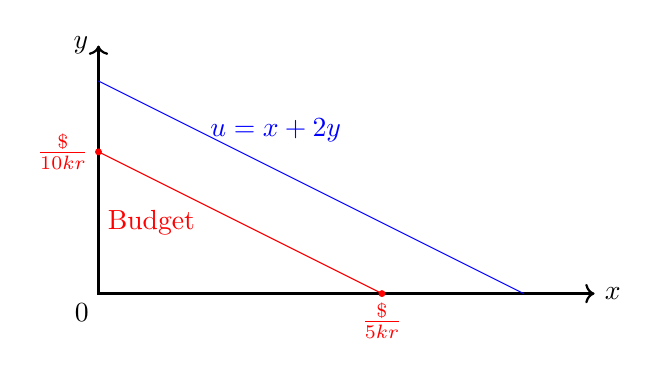
\begin{tikzpicture}[scale = 0.9]
\draw[thick,<->] (0,3.5) node[left]{$y$}--(0,0)--(7,0) node[right]{$x$};
\node [below left] at (0,0) {$0$};

\tkzDefPoint(0,0){O}
\tkzDefPoint(4,0){A}
\tkzDefPoint(0,2){B}
\tkzDefPoint(6,0){C}
\tkzDefPoint(0,3){D}

\draw [red] (B)--(A);
\draw [blue] (D)--(C) ;

\node[left,red] at (B) {$\frac{\$}{10 kr}$} ;
\draw[fill,red] (B) circle [radius =0.04];
\node[below,red] at (A) {$\frac{\$}{5 kr}$} ;
\draw[fill,red] (A) circle [radius =0.04];
\node[left,red] at (1.5,1) {Budget} ;
\node[above,blue] at (2.5,2) {$u = x + 2 y$} ;

\end{tikzpicture}
\captionof{figure}{A fair deal}
\label{fig:fair}
\end{center}
\vspace{2mm}

\begin{itemize}
\item $x$ : an apple , 5 kr per package.
\item $y$ : a 2-apple pack, 10 kr per package.
\end{itemize}

It's fair! Deb will not mind to substitute 2 $x$ with 1 $y$. Her demands lie on the budget frontier.

\vspace{2mm}

\textbf{Day 2:}

\begin{itemize}
\item $x$ : an apple , 5 kr per package.
\item $y$ : a 2-apple pack,\textcolor{red}{5 kr per package. On Sale!}.
\end{itemize}

\begin{center}
\begin{tikzpicture}
\draw[thick,<->] (0,5) node[left]{$y$}--(0,0)--(10,0) node[right]{$x$};
\node [below left] at (0,0) {$0$};

\tkzDefPoint(0,0){O}
\tkzDefPoint(4,0){A}
\tkzDefPoint(0,2){B}
\tkzDefPoint(8,0){C}
\tkzDefPoint(0,4){D}
\tkzDefPoint(0,4){E}
\tkzDefPoint(2,0){F}

\draw [red] (B)--(A);
\draw [red] (E)--(A);
\draw [dashed,red] (F)--(B);
\draw [blue] (D)--(C) ;

\node[left,red] at (B) {$\frac{\$}{10 kr}$} ;
\draw[fill,black] (B) circle [radius =0.04];
\node[left,red] at (E) {$\frac{\$}{5 kr}$} ;
\draw[fill,black] (E) circle [radius =0.04];

\node[below,red] at (A) {$\frac{\$}{5 kr}$} ;
\draw[fill,red] (A) circle [radius =0.04];

\node[left,red] at (1.9,1) {B} ;
\node[left,red] at (2.5,2) {B'} ;

\node[above,blue] at (4,2) {$u'$} ;


\end{tikzpicture}
\captionof{figure}{$y$ is on sale}
\label{fig:fair}
\end{center}
\vspace{2mm}

Deb will spend all income on $y$ because it's cheaper per apple. 

If Deb chose $(x=0,y=\frac{\$}{10 kr})$ in Day 1, when "relative price" changes (dash line), her demand 
will not change $\Rightarrow$ no substitution effects, and income effects only exist for $y$:

$$y = \frac{\$}{10kr} =  \to y= \frac{\$}{5kr}$$

(Note in Day 1, indifference curve $u$ is also on the budget frontier $B$)

\vspace{2mm}

\textbf{Day 3:}

\begin{itemize}
\item $x$ : an apple , \textcolor{red}{3 kr} per package (also on sale but still more expensive).
\item $y$ : a 2-apple pack,5 kr per package. Still on sale.
\end{itemize}
\begin{center}
\begin{tikzpicture}
\draw[thick,<->] (0,5) node[left]{$y$}--(0,0)--(9,0) node[right]{$x$};
\node [below left] at (0,0) {$0$};

\tkzDefPoint(0,0){O}
\tkzDefPoint(4,0){B}
\tkzDefPoint(8,0){C}
\tkzDefPoint(0,4){D}

\draw [red] (D)--(A);
\draw [red] (B)--(D);

\draw [red] (D)--(6,0);
\draw [blue] (C)--(D) ;

\node[left,red] at (D) {$\frac{\$}{5 kr}$} ;
\draw[fill,black] (D) circle [radius =0.04];
\node[below,red] at (A) {$\frac{\$}{5 kr}$} ;
\draw[fill,black] (A) circle [radius =0.04];

\node[left,red] at (3,2) {B''} ;
\node[below,red] at (2.5,1.5) {B'} ;

\node[below,blue] at (5.2,1.8) {$u'$} ;

\end{tikzpicture}
\captionof{figure}{$y$ is still cheaper}
\label{fig:fair}
\end{center}
\vspace{2mm}

There is no substitution effect and income effect  Demands unchange.

\vspace{2mm}

\textbf{Day 4:}

\begin{itemize}
\item $x$ : an apple , \textcolor{red}{2 kr} per package (Cheaper!).
\item $y$ : a 2-apple pack,5 kr per package. Still on sale.
\end{itemize}

\begin{center}
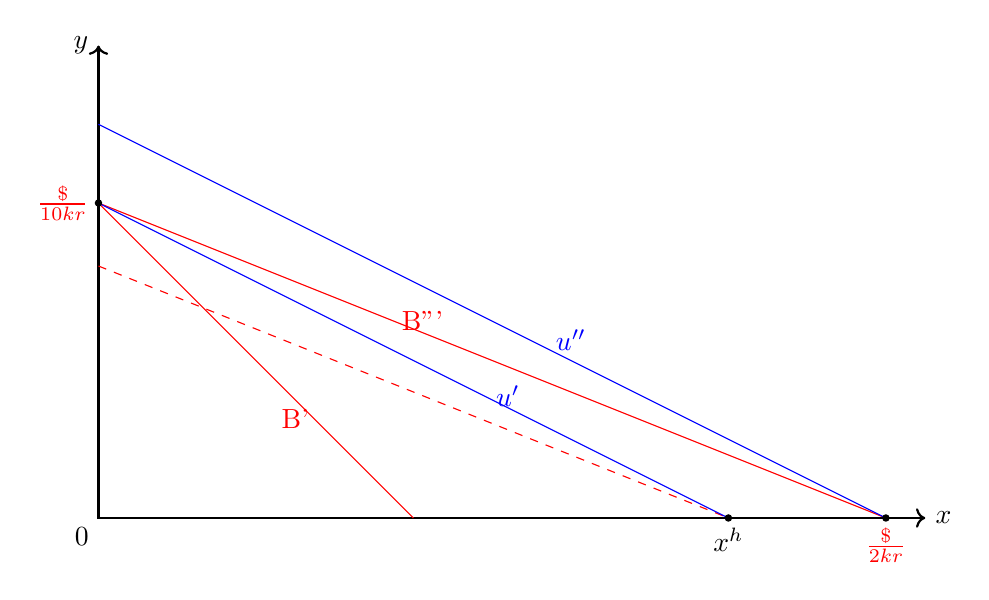
\begin{tikzpicture}
\draw[thick,<->] (0,6) node[left]{$y$}--(0,0)--(10.5,0) node[right]{$x$};
\node [below left] at (0,0) {$0$};

\tkzDefPoint(0,0){O}
\tkzDefPoint(10,0){A}
\tkzDefPoint(4,0){B}
\tkzDefPoint(8,0){C}
\tkzDefPoint(0,4){D}
\tkzDefPoint(0,5){E}

\draw [red] (D)--(A);
\draw [red] (B)--(D);

\draw [dashed,red] (0,3.2)--(C);
\draw [blue] (E)--(A) ;
\draw [blue] (C)--(D) ;

\node[left,red] at (D) {$\frac{\$}{10 kr}$} ;
\draw[fill,black] (D) circle [radius =0.04];
\node[below,red] at (A) {$\frac{\$}{2 kr}$} ;
\draw[fill,black] (A) circle [radius =0.04];
\node[below,black] at (C) {$x^h$} ;
\draw[fill,black] (C) circle [radius =0.04];

\node[left,red] at (4.5,2.5) {B'''} ;
\node[below,red] at (2.5,1.5) {B'} ;

\node[above,blue] at (6,2) {$u''$} ;
\node[below,blue] at (5.2,1.8) {$u'$} ;

\end{tikzpicture}
\captionof{figure}{$x$ is cheaper}
\label{fig:fair}
\end{center}

\vspace{2mm}


If the relative price changed (red dash line),with the same utility, Deb's demand will change:
$$x=0 \to x^h$$
$$y=\frac{\$}{10 kr} \to y= 0$$

This is due to substitution effect. In this case, the income effects only exist for $x$:
$$x^h \to x= \frac{\$}{2kr}$$

\end{mdframed}

Answer: The elasticity of substitution for Deb is infinite due to pefect substitution.

Assume there is a cheaper commodity, like $y$ in Day 2.
\begin{itemize}
\item When the cheaper is still cheaper($y$ in Day 3), no substitution effect, no income effect, no price effect.
\item When the cheaper becomes the more expensive ($y$ in Day 4),  income effect exists only for the cheaper ($x$ in Day 4).
\end{itemize}

\begin{mdframed}[backgroundcolor=yellow!20,linecolor=white]
Tips: Allocate your time according to the point of the questions.
\begin{itemize}
\item This is a 5\% point question, then just answer it briefly. 
\item Use graphs can save your time.
\item Use "common sense" to avoid proving (unless the question asks you to \textbf{calculate}), e.g. "straight" indifference curve  $\Rightarrow$ perfect substitution $\Rightarrow \sigma = + \infty $ 
\item Just skip it if you find it difficult. This small sub-question is really hard to answer.
\end{itemize}



\end{mdframed}

\begin{mdframed}[backgroundcolor=blue!20,linecolor=white]
Question: What is the implication of Leontief preference's ES for the income and substitution effects? 
\end{mdframed}

\newpage

Since you are here...
\section{exam 2019 Q1(c)-(d) - Choice with uncertainty}

\subsection{exam 2019 Q1(c) [5\%] }

c)Suppose that $x$ and $y$ measure the same commodity in two
different states of the world, say states $X$ and $Y$. 

\begin{itemize}
\item Rewrite the utility functions as expected utility functions. 
\item For which $\alpha$ do the utility functions for $D$ and $F$ have the same MRS at the 45 degree line?
\item What does this mean?
\end{itemize}

\begin{mdframed}[backgroundcolor=blue!20,linecolor=white]

The questiong want us to \textbf{rewrite} utility functions when there are 2 possible states. 

We know:
\begin{itemize}
\item The summation of the possibilities of the two states must be $1$.
\item Any monotonic transformation ($f(u)$ is a strictly increasing function of $u$, e.g. $f(u) = 0.5 u, f(u) = ln(u), f(u)=u^2 $) of utility functions will not change preference.
\end{itemize}
\end{mdframed}

1.Rewrite:

\begin{align*}
E(U_D) &= \frac{1}{3}x_D + {2}{3}y_D \\
E(U_F) &= \alpha ln x_F +  ({1-\alpha}) ln y_F 
\end{align*}

2.$\alpha$ and MRS:

\begin{align*}
MRS_{D12} &= 0.5 \\
MRS_{F12} &= \frac{\alpha / x}{({1-\alpha})/ y} = \frac{\alpha}{1-\alpha} \frac{y}{x} =  \frac{\alpha}{1-\alpha} \bigg\vert_{x=y}
\end{align*}

When $MRS_{D12} = 0.5 = MRS_{F12}\bigg\vert_{x=y} = \frac{\alpha}{1-\alpha}$, we have $\alpha = \frac{1}{3}$

3.Meaning

When $\alpha = \frac{1}{3}$, $E(U_F) =\frac{1}{3} ln x_F +  \frac{2}{3} ln y_F$ ,

Deb and Frank believe the possibilities of the two states are the same.

\subsection{exam 2019 Q1(d) [5\%] }

\begin{itemize}
\item Compute Deb's certainty equivalent at her endowment. 
\item Compute the Arrow-Pratt index of absolute risk aversion for Frank.
\end{itemize}

\begin{mdframed}[backgroundcolor=blue!20,linecolor=white]
\vspace{2mm}
{\centering
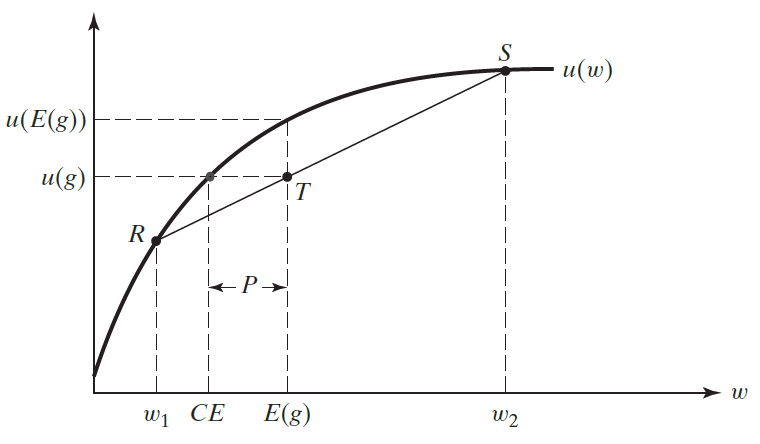
\includegraphics[width=0.8\textwidth]{4.cereq}
\captionof{figure}{Concave utility functions have positive risk premium $P \equiv E(g) - CE$}
\label{cf}}
\vspace{2mm}
\end{mdframed}

1. Deb's certainty equivalent

Since Deb's utility function $u = x$ is a straight line, $u[E(g)] = E(u)$,
$CE =  E(g) = 1$

2. Absolute risk aversion for Frank

\begin{mdframed}[backgroundcolor=blue!20,linecolor=white]
\textbf{DEFINITION 2.6 The Arrow-Pratt Measure of Absolute Risk Aversion}

$$R_a(w) \equiv -\frac{u''(x)}{u'(w)}$$

\end{mdframed}


The utility function of Frank with no uncertainty is $u = ln x$, thus

$$R_a(w) = -\frac{-\frac{1}{w^2}}{\frac{1}{w}}=\frac{1}{w}$$



\newpage

%%%%%%%%%%%%%%%%%%%%%%%%%%%%%%%%%%%%%%%%%%%%%%%%%%%%%%%%%%%%%%%%%%%%%%%%%%%%%%%%%%%%%%%%%%%%%%
\section{Jehle \& Reny 3.10}

A Leontief production function has the form $$y = min\{\alpha x_1, \beta x_2 \}$$
for $\alpha > 0$ and $\beta > 0$. Carefully sketch the isoquant map for this technology and verify that the
elasticity of substitution $\sigma = 0$, where defined.

\begin{mdframed}[backgroundcolor=blue!20,linecolor=white]
\begin{equation}
    \begin{cases}
If \ \alpha x_1 > \beta x_2, i.e. \frac{\alpha}{\beta}  x_1 >  x_2, y = \beta x_2 \\
If \ \alpha x_1 = \beta x_2, i.e. \frac{\alpha}{\beta}  x_1 =  x_2, y = \alpha x_1 = \beta x_2 \\
If \ \alpha x_1 < \beta x_2, i.e. \frac{\alpha}{\beta}  x_1 <  x_2, y = \alpha x_1
    \end{cases}
\nonumber
\end{equation}

Similar to Jehle \& Reny 1.27 in seminar 1, the indifference curves are seperated by a line. Here the line is
$\frac{\alpha}{\beta}  x_1 =  x_2$. Since $\alpha > 0$ and $\beta > 0, \frac{\alpha}{\beta} \in (0,+\infty)$

{\centering
\begin{tikzpicture}[scale=0.85]
\draw [->] (0,0) node [below] {0} -- (0,0) -- (6,0) node [below] {$x_1$};
\draw [->] (0,0) node [below] {0} -- (0,0) -- (0,3) node [left] {$x_2$};

\draw[dashed](0,0)--(5,2);
\node[right] at (5,2) {$x_2 = \frac{\alpha}{\beta}x_1$};
\node[right] at (1.5,2) {$y =  \alpha x_1$};
\node[right] at (3,0.8) {$y =\beta x_2$};

\end{tikzpicture}
\captionof{figure}{A possible $\frac{\alpha}{\beta}$}
\label{fig:3_10_1}}

We can then draw the indifference curves:

\end{mdframed}

{\centering
\begin{tikzpicture}[scale=0.85]
\draw [->] (0,0) node [below] {0} -- (0,0) -- (12,0) node [below] {$x_1$};
\draw [->] (0,0) node [below] {0} -- (0,0) -- (0,7) node [left] {$x_2$};

\draw [thick] (5,6) -- (5,2);
\draw [thick] (5,2) -- (11,2);
\draw [thick] (4,6) -- (4,1.6);
\draw [thick] (4,1.6) -- (11,1.6);

\draw [thick] (10,6) -- (10,4);
\draw [thick] (10,4) -- (11,4);

\draw[dashed](0,0)--(12,4.8);
\node[right] at (12,5) {$x_2 = \frac{\alpha}{\beta}x_1$};

\end{tikzpicture}
\captionof{figure}{A map of the indifference sets for Q.3.10}
\label{fig:3_10_2}}

\vspace{3mm}

Like Figure \ref{fig:leo}, when $\frac{x_2}{x_1}$ changes some angle $\gamma$, MRS changes from $+\infty$ to $0$.

$$MRTS = [\frac{d ln(MRTS)}{d ln(x_2/x_1)}]^{-1} =  [\frac{+\infty}{some \ finite \ number }]^{-1} = 0$$

\begin{mdframed}[backgroundcolor=blue!20,linecolor=white]
A formal proof: from CES to Leontief (read if you're interested)

\vspace{2mm}

Suppose we have a CES utility function:

$$u(x_1,x_2) = [(\alpha x_1)^\rho + (\beta x_2)^\rho]^\frac{1}{\rho}$$

Where $\rho < 1, and \ \rho \ne 0$. The Elasticity of Substitution of the CES utility function is $\sigma = \frac{1}{1-\rho}$ (Jehle \& Reny pp.130).


For simplicity, let's denote $\alpha x_1$ as $m$ and $\beta x_2$ as $n$. A log transformation will simplify our proof too:

$$ln u(m,n) = \frac{ln(m^\rho + n^\rho)}{\rho}$$

Then:

$$\lim_{\rho \to -\infty} ln u(m,n) = \lim_{\rho \to -\infty}\frac{ln(m^\rho + n^\rho)}{\rho} \to \frac{ln(0+0)}{-\infty} = \frac{\infty}{\infty}$$

Which is a \href{https://en.wikipedia.org/wiki/Indeterminate_form}{Indeterminate Form}. We can thus apply \href{https://en.wikipedia.org/wiki/L\%27H\%C3\%B4pital\%27s_rule}{L'Hôpital's rule}:

\begin{align*}
\lim_{\rho \to -\infty} ln u(m,n) &= \lim_{\rho \to -\infty}\frac{ln(m^\rho + n^\rho)}{\rho} \\
L'Hôpital's \ rule : \ \ \  &= \lim_{\rho \to -\infty} \frac{d ln(m^\rho + n^\rho) /d \rho}{d \rho / d\rho} \\
&= \lim_{\rho \to -\infty} \frac{m^\rho ln m+ n^\rho ln n}{m^\rho + n^\rho}
\end{align*}

(Note here we treat $\rho$ as the only variable, therefore $\frac{d x^\rho}{d\rho}=x^\rho lnx$)

Denote $c = min{m,n}$

\begin{align*}
\lim_{\rho \to -\infty} ln u(m,n) &=  \lim_{\rho \to -\infty} \frac{\frac{1}{c^\rho}}{\frac{1}{c^\rho}} ln u(m,n)\\
&= \lim_{\rho \to -\infty} \frac{(m/c)^\rho ln m+ (n/c)^\rho ln n}{(m/c)^\rho + (n/c)^\rho}
\end{align*}

\textbf{Case 1. if $m<n$}: $c = m, \frac{n}{c} = \frac{n}{m} >1$
\begin{align*}
\lim_{\rho \to -\infty} ln u(m,n) &= \lim_{\rho \to -\infty} \frac{1^\rho ln m+ (n/m)^\rho ln n}{1^\rho + (n/m)^\rho} \\
(\textcolor{red}{\frac{n}{m} >1}) \ \ \ \ \ \ \ &= \lim_{\rho \to -\infty} \frac{ln m+ 0}{1 + 0} \\
&= ln m 
\end{align*}

Therefore $\lim_{\rho \to -\infty} ln u(x_1,x_2) =ln m = ln (\alpha x_1) \Rightarrow \lim_{\rho \to -\infty} u(x_1,x_2) =  \alpha x_1$

\vspace{2mm}

\textbf{Case 2. if $m>n$}: $c = n, \frac{m}{c} = \frac{m}{n} >1$
\begin{align*}
\lim_{\rho \to -\infty} ln u(m,n) &= \lim_{\rho \to -\infty} \frac{(m/n)^\rho ln m+ 1^\rho ln n}{(m/n)^\rho + 1^\rho} \\
(\textcolor{red}{\frac{m}{n} >1}) \ \ \ \ \ \ \ &= \lim_{\rho \to -\infty} \frac{ 0 + ln n}{0 + 1} \\
&= ln m
\end{align*}

Therefore $\lim_{\rho \to -\infty} ln u(x_1,x_2) =ln n = ln (\beta x_2) \Rightarrow \lim_{\rho \to -\infty} u(x_1,x_2) =  \beta x_2$

\vspace{2mm}


To sum up, $$\lim_{\rho \to -\infty} u(x_1,x_2) = min\{\alpha x_1,\beta x_2\}$$

In addition, $$\lim_{\rho \to -\infty} \sigma =\lim_{\rho \to -\infty} \frac{1}{1-\rho} = 0$$

We can conclude:when $\rho \to -\infty$, the CES utility function shows Leontief preference, and $\sigma = 0$.
\end{mdframed}

%%%%%%%%%%%%%%%%%%%%%%%%%%%%%%%%%%%%%%%%%%%%%%%%%%%%%%%%%%%%%%%%%%%%%%%%%%%%%%%%%%%%%%%%%%%%%%
\section{Jehle \& Reny 3.11}
Calculate $\sigma$ for the Cobb-Douglas production function $y = Ax_1^\alpha x_2^\beta$, where $A > 0,\alpha > 0,$ and $\beta > 0$.

\begin{mdframed}[backgroundcolor=blue!20,linecolor=white]
$$\sigma_{12}(x_1,x_2) \equiv (\frac{d ln MRTS_{12}(r)}{dln r})^{-1}$$

$$ MRTS = \frac{\partial f(x_1,x_2) / \partial x_1}{\partial f(x_1,x_2) / \partial x_2}$$

\end{mdframed}

\begin{align*}
MRTS &= \frac{\partial  Ax_1^\alpha x_2^\beta / \partial x_1}{\partial  Ax_1^\alpha x_2^\beta / \partial x_2} \\
 &= \frac{A\alpha x_1^{\alpha - 1} x_2^\beta }{Ax_1^\alpha \beta x_2^{\beta -1}} \\
 &= \frac{\alpha x_2}{\beta x_1}
\end{align*}


Denote $\frac{x_2}{ x_1}$ as $r$, then $MRTS =  \frac{\alpha}{\beta} r$. Then,

\begin{align*}
\sigma_{12}&= (\frac{d ln (\frac{\alpha}{\beta} r)}{dln r})^{-1} \\
&= (\frac{d [ln (\frac{\alpha}{\beta}) +ln(r)]}{dln r})^{-1} \\
&= (\frac{d ln (\frac{\alpha}{\beta}) +d ln(r)}{d ln r})^{-1} \\
&= (\frac{0 +d ln(r)}{d ln r})^{-1} \\
& = 1
\end{align*}


%%%%%%%%%%%%%%%%%%%%%%%%%%%%%%%%%%%%%%%%%%%%%%%%%%%%%%%%%%%%%%%%%%%%%%%%%%%%%%%%%%%%%%%%%%%%%%
\section{Jehle \& Reny 3.14}

Calculate the elasticity of substitution for the production function in Example 3.2.

\begin{mdframed}[backgroundcolor=blue!20,linecolor=white]
EXAMPLE 3.2 (Jehle \& Reny  pp.134 ) A production function with variable returns to scale:
$$y = k(1 + x_1^{-\alpha} x_2^{-\beta} )^{-1}$$
where $\alpha > 0,\alpha > 0$, and $k$ is an upper bound on the level of output, so that $0 \le y < k$.
\end{mdframed}

\begin{align*}
MRTS &= \frac{\partial k(1 + x_1^{-\alpha} x_2^{-\beta} )^{-1} / \partial x_1}{\partial k(1 + x_1^{-\alpha} x_2^{-\beta} )^{-1} / \partial x_2} \\
 &= \frac{-k(1 + x_1^{-\alpha} x_2^{-\beta} )^{-2}(-\alpha) x_1^{-\alpha-1} x_2^{-\beta})}{-k(1 + x_1^{-\alpha} x_2^{-\beta} )^{-2} x_1^{-\alpha} (-\beta)x_2^{-\beta-1})} \\
 &= \frac{\alpha x_2}{\beta x_1}
\end{align*}

The same as Jehle \& Reny 3.11, $\sigma_{12} = 1$

\end{document}
